% !TeX root = ../数模通用模板.tex
\section{问题二的模型建立与求解}
\label{sec:q2-prediction}
问题二在每日0时确定全天购电量，负载和光伏则在运行中逐步揭晓。计划不足可能触发5倍电价的紧急补购，多购的剩余电量不能退款，因而预测的日内误差形状与储能的跨时段调节同样影响费用。本文以两类树模型融合预测供需，通过历史整日误差构造需求路径，依次确定充放电模式、修正购电量，再按当槽实况执行储能动作。

\subsection{负载与光伏的日前预测}
\subsubsection{历史特征与两类树模型融合}
将日内区间编号为$t=1,\ldots,144$，日期为$d$。每日0时仅使用此前已经观测到的负载和光伏，构造昨日、上周同槽、最近3日与7日均值、7日标准差，以及日内和星期周期特征，并加入昨日全日均值、标准差与极值，共31个特征。负载与光伏分通道训练直方图梯度提升树（HGB）和极端随机树（ExtraTrees），直接预测功率绝对值。

两个模型按月训练，月内参数冻结；每次训练均以该月开始前的完整历史日为依据。最近7日作为验证段，训练样本按90日半衰期加权。HGB最多100轮、15个叶节点，学习率0.08，叶节点至少50个样本，L2系数2，验证损失连续10轮未改善时停止；ExtraTrees使用128棵树，叶节点至少10个样本，不使用有放回抽样。两个模型的随机种子均为42。光伏非零时段由此前28日正发电时段的并集向两侧各扩展20分钟确定，预测值截为非负。

记通道$a\in\{\mathrm L,\mathrm V\}$的两个原始输出为$\widehat y_{d,t}^{a,H}$与$\widehat y_{d,t}^{a,E}$，先作等权融合：
\begin{equation}\label{eq:q2-forecast}
 \widehat y_{d,t}^{a,0}=\tfrac12\widehat y_{d,t}^{a,H}
 +\tfrac12\widehat y_{d,t}^{a,E}.
\end{equation}
式中，$d$为预测日期，$t$为日内10分钟区间编号；$a$为预测通道，$\mathrm L$和$\mathrm V$分别表示负载与光伏。$\widehat y_{d,t}^{a,H}$、$\widehat y_{d,t}^{a,E}$分别为HGB和ExtraTrees的原始功率预测，$\widehat y_{d,t}^{a,0}$为融合后的功率预测，单位均为kW；上标$0$标记尚未校准的输出。
融合权重对日期、时段和通道均固定，不根据当天实际误差选择模型。后续校准只作用于这一融合结果。

\subsubsection{共同岭回归校准与前日负载修正}
利用最近至多28个已完成日的原始融合误差，建立共同的输出校准。回归特征包括原始预测、昨日与上周及最近3日均值相对预测的偏差、另一通道的原始预测和日内谐波。功率特征除以1000后进入回归，历史日权重按14日半衰期衰减。对每个通道求
\begin{equation}\label{eq:q2-ridge}
 \widehat{\boldsymbol\beta}_{d}^{a}
 =\arg\min_{\boldsymbol\beta}\left\{
 \sum_{h\in\mathcal H_d}\sum_t\omega_h\nu_{h,t}^{a}
 \left[\frac{y_{h,t}^{a}-\widehat y_{h,t}^{a,0}}{1000}
 -(\mathbf x_{h,t}^{a})^{\mathsf T}\boldsymbol\beta\right]^2
 +\boldsymbol\beta^{\mathsf T}\Lambda\boldsymbol\beta\right\}.
\end{equation}
式中，$\mathcal H_d$为参与本次校准的最近至多28个已完成历史日，$h$为其中的日期索引，$\sum_t$遍历一天的144个区间。$y_{h,t}^{a}$为实测功率，$\mathbf x_{h,t}^{a}$为上述回归特征向量，$\boldsymbol\beta$为待估系数，$\widehat{\boldsymbol\beta}_{d}^{a}$为当日估计值；$\omega_h$为按14日半衰期衰减的日权重，$\nu_{h,t}^{a}$为槽内样本权重。$\Lambda$为对角惩罚矩阵，$\mathsf T$表示转置，$\arg\min$表示取使目标最小的系数；除以1000是功率的数值缩放。

$\Lambda$的截距惩罚为2，其余系数惩罚为20；负载样本权重$\nu=1$；历史光伏预测或实测值大于1\,kW的样本取权重1，其余取0.1。将回归修正恢复为kW，截断在$\max\{100,3\operatorname{RMSE}(r^a)\}$的正负范围内。这里$r^a$为该通道历史实测功率与原始融合预测之差的集合，$\operatorname{RMSE}$为均方根误差，$\max$取括号中的较大值，截断界限以kW计。再与原始预测相加、截非负并应用光伏时段限制，得到共同岭回归校准后的负载与光伏功率$\widetilde L_{d,t},\widetilde V_{d,t}$。无已完成校准样本时保留原始融合输出。

为补偿日平均负载偏差，再把前一日的平均残差按一半强度传递到当天：
\begin{equation}\label{eq:q2-memory}
 \widehat L_{d,t}=\max\left\{0,\widetilde L_{d,t}
 +\frac{1}{2T}\sum_{s=1}^{T}(L_{d-1,s}-\widetilde L_{d-1,s})\right\},
 \qquad \widehat V_{d,t}=\widetilde V_{d,t}.
\end{equation}
式中，$T=144$为每日区间数，$s$为前一日区间的求和索引，$L_{d-1,s}$为前一日实测负载功率；波浪号仍表示共同岭回归校准输出，$\widehat L_{d,t}$和$\widehat V_{d,t}$为最终发布的负载与光伏功率预测。系数$1/(2T)$表示取前日平均残差的一半。
这里的前日残差相对\emph{修正前}的共同岭回归输出计算，不使用已经叠加前日修正后的输出递归更新。没有相应前日预测时不加此项。

从1月1日开始采用同一条预测与调度流程。第1天用附件1作为已知先验；一月历史样本不足时，负载取上周同槽、未满一周取昨日同槽，光伏取昨日同槽。二月起使用上述树模型与校准输出。一月已完成日期的误差仍可进入后续历史路径集合，初始无历史日时采用一条零误差路径。该衔接不继承其他控制算法的储电轨迹。

\subsection{整日误差路径与日前调度}
\subsubsection{保留时间关联的需求路径}
净需求电量及其发布误差定义为
\begin{equation}\label{eq:q2-error}
 n_{d,t}=(L_{d,t}-V_{d,t})\Delta t,\qquad
 \widehat n_{d,t}=(\widehat L_{d,t}-\widehat V_{d,t})\Delta t,\qquad
 r_{d,t}=n_{d,t}-\widehat n_{d,t}.
\end{equation}
式中，$n_{d,t}$、$\widehat n_{d,t}$分别为实际与预测净需求电量，$r_{d,t}$为两者之差，单位均为kWh；$V_{d,t}$为实测光伏功率，$\Delta t=1/6$\,h为区间时长。功率差乘以$\Delta t$后换算为该区间电量。
在日$d$午夜，最近至多28个完整历史日组成$\mathcal H_d$，使用各历史日\emph{当时发布}的预测计算误差，而不是用当前模型重新解释过去。每个历史日形成一条144维路径：
\begin{equation}\label{eq:q2-paths}
 n_{d,t}^{(h)}=\widehat n_{d,t}+r_{h,t},\qquad h\in\mathcal H_d.
\end{equation}
式中，$n_{d,t}^{(h)}$为由历史日$h$的整日误差生成的当日净需求路径，上标$(h)$标记同一条场景路径中的各槽电量。
这种构造保留了一天内连续偏高或偏低的误差，能够反映储能量在多个时段积累偏差的影响。它与逐槽独立抽取分位点不同。

\subsubsection{模式规划与固定模式购电修正}
先按历史日顺序等间隔选取至多3条路径，建立共享购电量$g_t$和模式$m_t\in\{0,1\}$的情景混合整数规划。$m_t=1$允许充电，$m_t=0$允许放电。各路径的储能动作分别计算，并满足供需平衡、储电量上下界、功率限制以及与公共模式一致的约束。每日模式变化预算为
\begin{equation}\label{eq:q2-mode-budget}
 \sum_{t=1}^{T}|m_t-m_{t-1}|\leq8,
\end{equation}
式中，$m_t$为第$t$槽的公共计划模式，取1允许充电、取0允许放电；$m_{t-1}$为前一槽模式，$m_0$承接前一日的\emph{计划末模式}。$|m_t-m_{t-1}|$为相邻模式之差的绝对值，模式变化时取1，否则取0。因此跨午夜的变化也计入当天预算。模型最小保持时间为1槽。预算约束的是计划模式变化，不等同于实际非空动作的反转次数。

模式规划的代理目标为
\begin{equation}\label{eq:q2-plan-objective}
 J_{\rm MIP}=\sum_tp_tg_t+
 \frac1K\sum_{h=1}^{K}\left[
 \sum_t\{5p_te_t^{(h)}+0.002(c_t^{(h)}+d_t^{(h)})\}
 -v_{\rm MIP}(E_{T+1}^{(h)}-1200)\right].
\end{equation}
式中，$J_{\rm MIP}$为模式规划的代理费用，$p_t$为已知的分时电价，单位为元/kWh；$g_t$为各路径共享的计划购电量，单位为kWh。$K$为选入规划的路径数，最多取3，此处将所选路径重编号为$h=1,\ldots,K$。$e_t^{(h)}$、$c_t^{(h)}$和$d_t^{(h)}$分别为路径$h$的紧急购电量、充电量和放电量，均按外部电量计，单位为kWh；$E_{T+1}^{(h)}$为该路径的日末内部储电量。$v_{\rm MIP}$为每kWh期末库存的估值，1200为最低内部储电量，系数5为紧急购电加价倍数，0.002为每kWh充放电吞吐的代理权重。

普通日取$v_{\rm MIP}=\min_t p_t/\eta_c$，其中$\min_t$取当日最低电价，$\eta_c$为充电单向效率；年末最后一天取0。路径中的未来动作辅助评价这一共同计划，真实运行时则逐槽重新计算储能反馈。

第二步固定求得的整日模式，在全部至多28条历史路径上，按下节相同的储能反馈公式回放，使用L-BFGS-B调整144个非负购电量。修正目标仍计计划费、平均紧急费和0.002元/kWh的吞吐权重，普通日的期末库存估值改为0.45元/内部储电kWh，12月31日取0。至此购电计划锁定，实际运行不再改变当天$g_t$。这一数值修正求得局部解，其代理目标值及单日MIP间隙都不构成全年实际费用的全局最优保证。

\subsection{实际执行、结算与实现边界}
\subsubsection{按当槽实况反馈}
执行时令$B_t=g_t+(V_t-L_t)\Delta t$。在区间内快速测量与反馈的假设下，使用当槽实际供需计算
\begin{equation}\label{eq:q2-execute-charge}
 c_t=m_t\min\{(B_t)^+,P_{\max}\Delta t,(E_{\max}-E_t)/\eta_c\},
\end{equation}
式中，$B_t$为计划购电与实际净供电合成后的槽内电量余缺，正值表示有余电；$c_t$为实际充电量，$P_{\max}$为充放电功率上限（kW），$E_t$和$E_{\max}$分别为槽初内部储电量及其上限（kWh）。$(B_t)^+$表示取$B_t$与0中的较大值，$\min$取括号中各项的最小值；本节单日调度式省略日期下标$d$。
\begin{equation}\label{eq:q2-execute-discharge}
 \begin{aligned}
 d_t&=(1-m_t)\min\{(-B_t)^+,P_{\max}\Delta t,(E_t-E_{\min})\eta_d\},\\
 e_t&=(-B_t-d_t)^+,\qquad w_t=(B_t-c_t)^+.
 \end{aligned}
\end{equation}
式中，$d_t$、$e_t$和$w_t$分别为实际放电量、紧急购电量和剩余电量，单位为kWh；$E_{\min}$为内部储电量下限，$\eta_d$为放电单向效率。上标$+$在各式中均表示取正部。
实际动作受模式、余缺电量、容量和功率约束，不再以规划场景的意图充放电量作为上限，充电死区取0。随后更新
\begin{equation}\label{eq:q2-balance}
 E_{t+1}=E_t+\eta_c c_t-d_t/\eta_d,\qquad
 g_t+e_t+d_t=n_t+c_t+w_t.
\end{equation}
式中，$E_{t+1}$为该槽结束后的内部储电量，$n_t$为省略日期下标后的实际净需求电量。
该规则不会同时充放电，也不会用紧急购电给电池充电。$w_t$包含已付费但未利用的计划电量与未利用光伏，未区分来源时只报告总剩余电量。

\subsubsection{真实费用与跨日状态}
问题二的真实购电费仅为
\begin{equation}\label{eq:q2-real-cost}
 C=\sum_{d,t}p_tg_{d,t}+5\sum_{d,t}p_te_{d,t}.
\end{equation}
式中，$C$为统计区间内的实际购电总费用（元），$\sum_{d,t}$遍历该区间的全部日期和日内时槽；$g_{d,t}$、$e_{d,t}$为恢复日期下标后的计划与紧急购电量，下文用$J$统称规划代理目标。
吞吐权重和期末库存估值只出现在规划目标$J$中，不进入$C$，也不形成售电或残值收益。运行从2025年1月1日6000\,kWh起步，每日承接上一日的实际末储电量、计划末模式及其已保持槽数。普通日不要求储电量回到6000\,kWh。表\ref{tab:q2-setup}汇总具体实现。
\begin{table}[H]\centering\small
\caption{问题二的规划、修正与执行设置}\label{tab:q2-setup}
\begin{tabularx}{\textwidth}{p{3.6cm}X}\toprule
环节&设置\\\midrule
供需预测&原始HGB/ExtraTrees等权融合；共同28日岭回归校准；非递归前日负载残差的一半。\\
历史路径&最近至多28个已完成日的整日误差；模式规划等间隔选至多3条，购电修正使用全部路径。\\
模式规划&10分钟共模，最短保持1槽，每天含午夜边界最多8次变化；无换向软罚，吞吐权重0.002元/kWh。\\
求解预算&MIP每次最多5\,s，目标相对间隙0.2\%；L-BFGS-B最多120次迭代，记录真实停止状态。\\
期末估值&MIP取当日最低预测价除以单向效率；固定模式修正取0.45元/kWh；末日均取0。\\
实际执行&当槽供需反馈，死区0，无意图电量上限；全年实际储电量连续。\\
跨日状态&实际储电量、计划末模式、该计划模式已保持槽数。\\
输出范围&控制运行365日；附件5工作簿取2月1日到12月31日334日、48096槽。\\
\bottomrule\end{tabularx}\end{table}

\subsection{指定日期、全年费用与结果检验}
按题目给定日期和时段，表\ref{tab:q2-purchase-dates}并列四个日期的计划购电量与全天费用；表\ref{tab:q2-battery-20250320}和表\ref{tab:q2-battery-20250621}、表\ref{tab:q2-battery-20250923}和表\ref{tab:q2-battery-20251221}分别并排给出实际充放电量及起止储电量，表\ref{tab:q2-emergency}给出连续紧急购电区间。所报计划购电量是0时锁定值，全天费用含紧急补购；电量以kWh计并保留四位小数，金额以元计并保留两位小数。时间段使用左闭右开区间，四小时量按其包含的24个槽相加。
\begin{table}[H]\centering\small
\caption{2025年四个指定日期的计划购电量及全天费用}\label{tab:q2-purchase-dates}
\begin{tabular}{lrrrr}\toprule
时间段或指标&3月20日&6月21日&9月23日&12月21日\\\midrule
10:00--10:10&48.2652&0.0000&0.0000&45.6628\\
12:00--12:10&606.0250&0.0000&491.0172&948.0275\\
14:00--14:10&0.0000&0.0000&0.0000&0.0000\\
16:00--16:10&439.5483&220.1115&503.9053&868.6242\\
18:00--18:10&673.0022&132.0644&746.5827&684.9746\\
20:00--20:10&25.2301&0.0000&127.3036&33.5085\\
\midrule
全天计划购电量/kWh&65277.1470&30903.9138&67847.2652&93111.4419\\
全天购电费/元&40076.53&19195.23&43261.35&60110.89\\
\bottomrule\end{tabular}\end{table}
\begin{table}[H]\centering\small
\caption{2025年四个指定日期的充放电量及起止储电量（kWh）}\label{tab:q2-battery-dates}
\begin{tabular}{lrrrr}\toprule
时间段或指标&3月20日&6月21日&9月23日&12月21日\\\midrule
\multicolumn{5}{l}{充电量（kWh）}\\
00:00--04:00&6395.6805&0.0000&7093.1118&7517.4410\\
04:00--08:00&2500.0565&787.9293&716.6349&3426.9275\\
08:00--12:00&5809.0850&10119.2885&5277.7118&5176.1069\\
12:00--16:00&3657.8022&0.0000&2459.3218&6372.7058\\
16:00--20:00&400.6455&0.0000&0.0000&0.0000\\
20:00--24:00&1150.3048&2055.9982&1918.6147&0.0000\\
\midrule
\multicolumn{5}{l}{放电量（kWh）}\\
00:00--04:00&0.0000&1438.8347&0.0000&0.0000\\
04:00--08:00&6254.0246&3286.6826&4990.4167&2445.3267\\
08:00--12:00&2732.1701&0.0000&1896.6157&6897.5587\\
12:00--16:00&671.0733&0.0000&407.6353&2685.3895\\
16:00--20:00&5806.4536&5634.7636&6126.8605&5941.8612\\
20:00--24:00&2818.9397&3340.3250&2778.3055&2895.6742\\
\midrule
0:00储电量&2851.9662&5433.6372&3391.0237&2140.0098\\
24:00储电量&2472.0243&3289.9172&2884.0282&1484.4197\\
\bottomrule\end{tabular}\end{table}
\begin{table}[H]\centering\small
\caption{四个指定日期的连续紧急购电区间及电量}\label{tab:q2-emergency}
\setlength{\tabcolsep}{3pt}\begin{tabular}{lrlrlrlr}\toprule
\multicolumn{2}{c}{3月20日}&\multicolumn{2}{c}{6月21日}&\multicolumn{2}{c}{9月23日}&\multicolumn{2}{c}{12月21日}\\
时间段&电量&时间段&电量&时间段&电量&时间段&电量\\\midrule
01:00--01:20&14.9026&06:40--07:20&247.6871&14:50--15:10&20.5010&03:30--03:50&73.6481\\
--&--&--&--&20:50--21:00&26.1799&10:40--10:50&36.2066\\
\bottomrule\end{tabular}\end{table}
表\ref{tab:q2-annual}同时给出全年账单与附件5要求区间的账单，二者不混用。
\begin{table}[H]\centering\small
\caption{问题二不同统计区间的购电量与实际费用}\label{tab:q2-annual}
\begin{tabular}{lrr}\toprule 指标&1--12月（365日）&2--12月（334日）\\\midrule
计划购电量/kWh&23465106.4174&20519293.0944\\
紧急购电量/kWh&154624.4448&104033.4282\\
外网合计购电量/kWh&23619730.8622&20623326.5225\\
计划购电费/元&14518936.61&12636712.82\\
紧急购电费/元&811967.83&558940.83\\
合计费用/元&15330904.44&13195653.64\\
\bottomrule\end{tabular}\end{table}
预测误差采用2--12月每日午夜最终输出，所有槽各计一次，样本数均为48096；结果见表\ref{tab:q2-prediction}。MAE为平均绝对误差，RMSE为均方根误差，偏差取预测功率减实测功率的均值。
\begin{table}[H]\centering\small
\caption{午夜最终供需预测的误差（2--12月，不重叠日窗口）}\label{tab:q2-prediction}
\begin{tabular}{lrrr}\toprule 变量&MAE/kW&RMSE/kW&偏差/kW\\\midrule
负载&136.9731&182.9870&-3.5806\\
光伏&153.2594&307.0504&6.1798\\
净负载&242.0206&357.1618&-9.7604\\
\bottomrule\end{tabular}\end{table}

全年实际购电费为15330904.44元，其中1月费用为2135250.79元，2--12月费用为13195653.64元。2月1日初始储电量为3743.6008\,kWh，由一月同一策略的实际末状态连续承接，未重新设为6000\,kWh。四个指定日期共出现6个连续紧急购电区间；购电不足由紧急补购补齐后，全部52560槽均满足供需平衡、功率与储电量约束。

2--12月实际非空方向反转为2535次，活动槽为37259个，交流侧充放电吞吐为11340559.8068\,kWh。反转先剔除空闲动作，再在评价区间内部连续计数，不计入一月与二月的连接边界。这些量分别反映运行强度的不同侧面，不将计划模式变化预算解释为所有实际动作指标都会下降。

365次模式规划均取得可行解，其中113次达到求解时限，最大实际相对间隙为7.5327\%；固定模式修正中60次按求解器成功条件停止。模式规划累计耗时1043.50\,s，购电修正累计耗时640.54\,s；这些是各阶段求解累计时间，不包含模型训练与制图，也不是多进程运行的总墙钟时间。实际账单逐槽复算最大残差为9.09e-13元。

图\ref{fig:q2-monthly}按月给出计划费与紧急费的构成，用于观察各月账单和补购负担。柱形为月总费用，包含当月天数及季节需求共同影响，不将其直接解释为单位时间调度效率。
\begin{figure}[H]
 \centering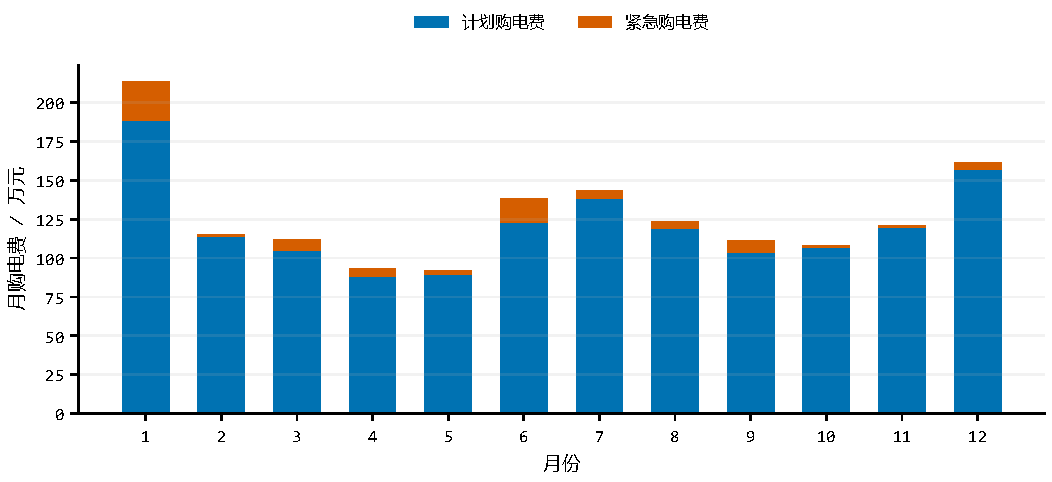
\includegraphics[width=\textwidth]{final_results/q2/q2_monthly.pdf}
 \caption{问题二全年各月计划购电费与紧急购电费}\label{fig:q2-monthly}
\end{figure}
该结果属于按时间推进的开发年度回测：预测发布只用历史信息，2025年数据同时参与过方法开发与选择，因而不能据本年度结果声称独立跨年泛化能力。固定随机种子42得到的树模型结果，也不替代多种子稳定性检验。
